%%%%%%%%%%%%%%%%%%%%%%%%%%%%
\documentclass[a4paper,11pt,spanish]{report}
%%%%%%%%%%%%%%%%%%%%%%%%%%%%
% LINE SPACING
\newcommand{\linespacing}{1.5}
\renewcommand{\baselinestretch}{\linespacing}
%%%%%%%%%%%%%%%%%%%%%%%%%%%%
%%%%%%%%%%%%%%%%%%%%%%%%%%%%
%BIBLIOGRAPHY STYLE
\usepackage{natbib}
\bibliographystyle{plain}
% \bibliographystyle{plain} for [1], [2] etc.
%%%%%%%%%%%%%%%%%%%%%%%%%%%%

%%%%%%%%%%%%%%%%%%%%%%%%%%%%
% OTHER FORMATTING/LAYOUT DECLARATIONS
% Graphics
\usepackage{algorithm}
\usepackage[noend]{algpseudocode}
\makeatletter
\def\BState{\State\hskip-\ALG@thistlm}
\makeatother

\usepackage[noend]{algpseudocode}
\usepackage{graphicx,color}
\usepackage[english]{babel}
\selectlanguage{English}
\usepackage[utf8]{inputenc}
\usepackage{listings}
\usepackage{amsmath}
\usepackage{microtype}
\usepackage{enumitem}
%\usepackage{minted}
\usepackage{longtable}
\usepackage{booktabs}
\usepackage{epstopdf}
%\usepackage[british]{babel}
% The left-hand-side should be 40mm.  The top and bottom margins should be
% 25mm deep.  The right hand margin should be 20mm.
\usepackage[a4paper,top=2.5cm,bottom=2.5cm,left=2.7cm,right=2.5cm,headsep=10pt]{geometry}
%\flushbottom
% Pages should be numbered consecutively through the main text.  Page numbers
% should be located centrally at the top of the page.
\usepackage{fancyhdr}
\fancypagestyle{plain}{
	\fancyhf{}
	% Text in header
 	%\lhead{\textit{\today}}
	%
	\cfoot{\thepage}
	\renewcommand{\headrulewidth}{0pt}
}
% Paragraph separation and indents
\pagestyle{plain}
\setlength{\parskip}{\baselineskip}%
\setlength{\parindent}{0pt}
%%%%%%%%%%%%%%%%%%%%%%%%%%%%

%%%%%%%%%%%%%%%%%%%%%%%%%%%%
% HYPER REF
\usepackage[colorlinks,pagebackref,pdfusetitle,urlcolor=black,citecolor=black,linkcolor=black,bookmarksnumbered,plainpages=false]{hyperref}
% For print version, use this instead:
%\usepackage[pdfusetitle,bookmarksnumbered,plainpages=false]{hyperref}
%\usepackage{backref}
%\renewcommand{\backrefpagesname}{Cited on}
%%%%%%%%%%%%%%%%%%%%%%%%%%%%

%%%%%%%%%%%%%%%%%%%%%%%%%%%%
% BEGIN DOCUMENT
\begin{document}
\raggedbottom
%%%%%%%%%%%%%%%%%%%%%%%%%%%%

%%%%%%%%%%%%%%%%%%%%%%%%%%%%
% PREAMBLE: roman page numbering i, ii, iii, ...
\pagenumbering{roman}
%%%%%%%%%%%%%%%%%%%%%%%%%%%%

%%%%%%%%%%%%%%%%%%%%%%%%%%%%
%% TITLE PAGE: The title page should give the following information:
%%	(i) the full title of the thesis and the sub-title if any;
%%	(ii) the full name of the author;
%%	(iii) the qualification aimed for;
%%	(iv) the name of the University of Sussex;
%%	(v) the month and year of submission.
\thispagestyle{empty}
\begin{flushright}
\includegraphics[width=6cm]{figures/LOGO_ESCUELA}
\end{flushright}
\vskip40mm
\begin{center}
% TITLE
\huge\textbf{Development of unsupervised learning transformations through supervised learning methods.}
\vskip2mm
% SUBTITLE (optional)
\LARGE\textit{}
\vskip5mm
% AUTHOR
\Large\textbf{Author: Patricia Cortajarena Sauca}

\Large\textbf{Ponente: Carlos Roberto del Blanco Adán}

\Large\textbf{Tutor: Iñigo Cortajarena Sauca}

\end{center}
\vfill
\begin{flushleft}
\large
% QUALIFICATION
Trabajo Fin de Grado \\
ETSIT UPM 	\\
% DATE OF SUBMISSION
Madrid. January, 2018
\end{flushleft}
%%%%%%%%%%%%%%%%%%%%%%%%%%%%

%%%%%%%%%%%%%%%%%%%%%%%%%%%%
% ABSTRACT
\chapter*{Abstract}
\setcounter{page}{3}

The aim of this project is  


%%%%%%%%%%%%%%%%%%%%%%%%%%%%
% ACKNOWLEDGEMENTS
\chapter*{Acknowledgements}

\renewcommand{\baselinestretch}{\linespacing}
\small\normalsize
% ACKNOWLEDGEMENTS HERE:
%%%%%%%%%%%%%%%%%%%%%%%%%%%%%

%%%%%%%%%%%%%%%%%%%%%%%%%%%%%
% TABLE OF CONTENTS, LISTS OF TABLES & FIGURES
\newpage
\pdfbookmark[0]{Contents}{contents_bookmark}
\tableofcontents
\listoftables
\phantomsection
\addcontentsline{toc}{chapter}{List of Tables}
\listoffigures
\phantomsection
\addcontentsline{toc}{chapter}{List of Figures}
%%%%%%%%%%%%%%%%%%%%%%%%%%%%%

%%%%%%%%%%%%%%%%%%%%%%%%%%%%%
% MAIN THESIS TEXT: arabic page numbering 1, 2, 3, ...
\newpage
\pagenumbering{arabic}
%%%%%%%%%%%%%%%%%%%%%%%%%%%%%

%-----------------------------------------------------
% Chapter: Introduction
%-----------------------------------------------------

\chapter{Introduction}
\label{chap:intro}

Working with large datasets and high-dimensional data in nowadays' problems has encouraged the use of dimensionality reduction algorithms which try to preserve as much information as possible even with a reduced number of features used to describe that same dataset. This means  dimensionality reduction algorithms compute new features based on the original ones. Although the number of new features computed are less than the number of original ones, the reduction's objective is to still represent the same information without significant distortion. Thus, time and memory in huge implementations are saved.

Taking into account that this turns into a difficult task, numerous approaches have been proposed.\\
Although the different approaches try to achieve more or less the same aim, they differ from one another and we can not reassure which would suite for a specific problem or even if the behaviour of the algorithm throws the results we expected or needed.

The first point to take into account is the existence of parametric and non-parametric algorithms, depending on whether the dimensionality reduction can be expressed in terms of parameters or not, which can be conclusive when deciding what algorithm to use.\\
Secondly, in both of them we can find different models proposed depending on what to optimize, yet not everything is going to be preserved as well as in the original dataset, so we need to prioritize some aspects.

So the decision of which of them to implement depends on the previous study of our data, the performance requirements and the later purpose and usage of the reduced data.

The non-parametric algorithms have an important disadvantage: as it is said, they don't have parameters which represent the dimensionality reduction; thus, when a new datapoint is provided we need to compute the whole algorithm again to obtain the datapoint's representation in the lower space, instead of computing only the new data.

We hereby propose the study and research of an implementation which replicates the behaviour of a non-parametric dimensionality reduction algorithm. The main objective is to solve the non-parametric's main disadvantage and make the new algorithm capable of being repeatedly used with new datapoint examples, omiting the need to compute the whole dimensionality reduction algorithm every time.\\
The dimensionality reduction algorithms used to base the research are the ones listed below:
\renewcommand{\labelitemi}{\textendash}
\begin{itemize}
\item PCA (Principal Component Analysis)
\item MDS (Multidimensional Scaling)
\item TSNE (T-Stochastic Neighbour Embedding)
\end{itemize}

To conclude, the document is divided into chapters which resume the main steps of this research. Chapter number \ref{chap:stt} describes the State-of-The-Art. It is followed by chapter \ref{chap:frame}, which details the main development of the implementation. Afterwards, chapters \ref{chap:app} and \ref{chap:met} describe the main implementation's applications and the corresponding metrics computed to analyse the algorithm's behaviour. The last chapter (chapter \ref{chap:conc}) comprehends the conclusion and resumes the main ideas acquired.

%-----------------------------------------------------
% Chapter: State of the Art
%-----------------------------------------------------

\chapter{State-of-The-Art}
\label{chap:stt}

The most classical dimensionality reduction techniques are know to be PCA \citep{pca} and MDS \citep{mds}. They preserve the true structure of the data even though they are simple to implement and efficiently computable. They rely on linear models to compute data mining on near lower dimensional spaces. A related linear implementation which is based on random projectations of the data is described in \citep{rproj, rproj2}. Some other well-known techniques are ISOMAP \citep{isomap} and t-SNE \citep{tsne}, but their implementations often require more memory and computational time, yet the complexity of the algorithms is higher. Nevertheless, this algorithms are capable of reducing the number of features in non-linear data, where linear models can not faithfully reprensent the data's structure. ISOMAP computes geodesic distances instead of taking into account only euclidean distances while t-SNE's approach calculates probabilities from euclidean distances.

Neural networks have become an essencial tool in machine learning problems and it is certainly used in dimensionality reduction. The autoencoders \citep{auto2, auto} consist on a neural net with decreasing number of neurons per layer and then symmetrically more layers are added with the same corresponding increasing neurons per layer. If the output represents without distorsion the input to the net, the middle layer with the fewest number of neurons corresponds to the reduced description of the data. This is represented in figure \ref{autoencoder}.

\begin{figure}[h]
\centering
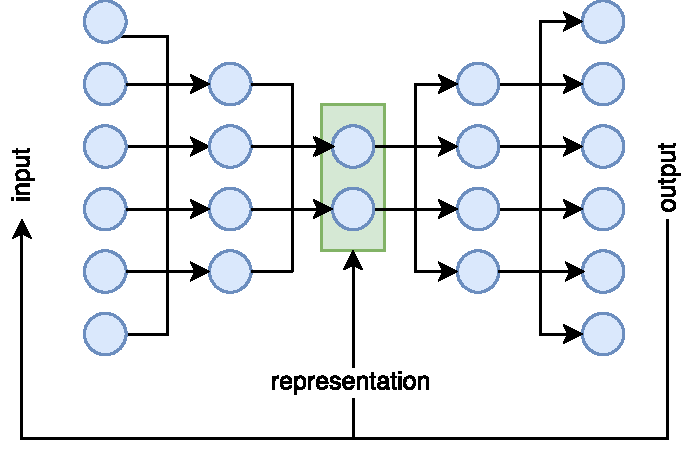
\includegraphics[width=8cm]{figures/autoencoder.pdf}
\caption{\label{autoencoder}Autoencoder neural network.}
\end{figure}

The next sections (sections \ref{sec:pca}, \ref{sec:mds} and \ref{sec:tsne}) resume the main ideas of the algorithms in which the research is based. 

\section{PCA: Principal Component Analysis}
\label{sec:pca}

Principal Component Analysis \citep{pca} algorithm is based on reducing the number of features by processing the correlations between the features of the datapoints. The aim is to eliminate this correlations by transforming the matrix \textbf{X} $\in$ $\Re^{mxn}$ (with m being the number of data points and n de number of features) into an orthogonal basis. By omiting the correlation between columns of the matrix \textbf{X} we are capable of doing away with redundancies.\\
The model starts by computing de covariance matrix, which results in a $\Re^{nxn}$ symmetric matrix. We obtain it by using the next expression:
\begin{center}
cov(\textbf{X}) = $\dfrac{1}{m-1}$ $\textbf{X}^{T}$\textbf{X}
\end{center}
Because the aim of the PCA is to eliminate the correlations, the covariance matrix of the result \textbf{Y} should be a diagonal matrix with just the variances of the columns.\\
PCA is famous because of a great advantage: we can find a linear transformation (\textbf{Y = XP}), which makes this a parametric model, easy to reuse and quite computationally simple.\\
For symmetric matrices (\textbf{X}) we can find eigenvalue decomposition with a diagonal matrix (\textbf{Y}), matching exactly with our linear problem with \textbf{X} and \textbf{Y}.
\begin{center}
\textbf{Y = XP}
$$ cov(\textbf{Y}) = \frac{1}{m-1} \textbf{Y}^{T} \textbf{Y} = \frac{1}{m-1} \textbf{(XP)}^{T} \textbf{XP} = \textbf{P}^{T} cov(\textbf{X})\textbf{P} $$
$$\textbf{D} = \textbf{V}^{T} \textbf{AV}$$
$$ \textbf{A} = cov(\textbf{X}); \textbf{P} = \textbf{V}^{T}; \textbf{D} = cov(\textbf{Y})$$
\end{center}

With the previous expressions we get to the point that, by computing the eigenvectors of the covariance matrix \textbf{X}, we can get a linear transformation from space \textbf{X} to space \textbf{Y}. The eigenvalues matrix obtained (cov(\textbf{Y})) are sorted decreasingly and are the orthogonal basis values. Choosing the \textbf{N} first values of this matrix, being \textbf{N} the desired output dimension, and computing the corresponding eigenvectors, we obtain our reduced dimensionally points, as a basis transformation of our datapoints from the original dataset, by the new basis coordinates.

\section{MDS: Multidimensional Scaling}
\label{sec:mds}

Multidimensional Scaling \citep{mds} in dimensionality reduction tries to create a map which displays the relative distances between the data points. This focuses on getting a lower dimensional map, keeping as much distance information as possible. In case of visualizing data, this dimensional map needs to be a one, two or, at most, three dimensional space.\\
MDS calculates a metric or non-metric solution depending on the data provided, which has to be a \textit{proximity} matrix. This \textit{proximity} matrix quantifies how close the datapoints are. On the one hand for metric solutions, this \textit{proximity} matrix has to be a true distance matrix, while on the other, both dissimilarities or correlations are alternatives to the input for the problem's matrix.

MDS algorithm is based on some ideas explained in the previous section. The \textit{proximity} matrix is always  symmetric and somehow describes the relations between the features, so basically we can treat our problem as a variation of the PCA algorithm.\\
Metric MDS performs the same steps as in PCA, with the modification of being a distance matrix the one computed in this problem.\\
In non metric MDS, we assume a less strict relation and we compute the observed distances as a function of the real distance plus some meassure error. The usable information in this case is going to be the rank order of the previous matrix, which could be the input for the model.\\
The main difference between PCA and MDS is the fact that, because of the need to compute a pairwise distance or proximity matrix, there is no linear transformation that suits both the distance computations plus the matrix operations, so MDS turns to be non-parametric.

\subsection{Stress metric}
\label{ssec:str}

As in every data problem, we need a metric which shows how well the performance given a particular dataset is. In Multidimensional Scaling we compute the \textit{stress} measure that compares the predicted distances with the original ones. Note that obviously this depends on the number of dimensions we want to keep, yet if we lower the number of dimensions, the stress will get higher, because we are representing the same distances relations in a lower dimensional space.
\begin{center}
\( \textit{stress} = \sqrt{\frac{\sum(d_{ij}-d'_{ij})^{2}}{\sum d_{ij}^{2}} } \)
\end{center}
$d_{ij}$ represents the original distance and $d'_{ij}$ is the predicted distance based on the MDS model. This last value is either a predicted distance or a function which represents the non-metric transformation of the data.\\
Regarding the previous expression, if our prediction stands well for the original data, the stress value should lower, relating zero stress to the perfect performance of the MDS  algorithm. 

\section{TSNE: T-Stochastic Neighbour Embedding}
\label{sec:tsne}

T-Stochastic Neighbour Embedding \citep{tsne} is our non-linear example of dimensionality reduction. It relies on Stochastic Neighbour Embedding (SNE). The main reason why this algorithm is used is because it is capable of representing both the local and the global structure of the original data. As said, this section will be divided in two: the basis SNE and the T-SNE upgrades.

\subsection{SNE}
\label{ssec:sne}

SNE approaches the dimensionality reduction by converting the Euclidean distances into conditional probabilities as a way of expressing similarities between points. That means we measure the similarity of two points $x_{i}$, $x_{j}$ as the probability $p_{i|j}$ of considering the second one as a neighbour of the first. The probability in the original and in the low dimensional space is computated as seen:

$$ p_{i|j} = \frac{exp(-||x_{i}-x_{j}||^{2}/2\sigma_{i}^{2})}{\sum _{k\neq i} exp (-||x_{i}-x_{k}||^{2}/2\sigma_{i}^{2})}$$

$$ q_{i|j} = \frac{exp(-||y_{i}-y_{j}||^{2})}{\sum _{k\neq i} exp (-||y_{i}-y_{k}||^{2})} $$

This expressions represent gaussian distributions centered in each datapoint $x_{i}$, where $\sigma_{i}$ is the example's variance. The conditional probability represents whether the point $x_{j}$ is considered a datapoint's neighbour or not. According to the value of $\sigma_{i}$ the probabilities change, so it is chosen depending on the density of the data. In a dense region, a smaller value of $\sigma_{i}$ is more appropiate than in a sparse region. Having decided which value to use for each of the datapoints, we obtain a probability distribution, $P_{i}$, that is computed as explained in the next paragraph.

As the point of this metric is to compute similarities as probabilities, we can calculate the mismatch between $p_{i|j}$ and $q_{i|j}$ with all the datapoints and consequently obtain the algorithm's behaviour by analysing how many neighbours have been mantained in the low dimensional map. In terms of conditional probabilities, Kullback-Leibler divergence perfectly suits this need. Summing up all the previous ideas we get to the point of minimizing the cost function described as:

$$ C = \sum\limits_{i} KL(P_{i}||Q_{i}) = \sum\limits_{i} \sum\limits_{j} p_{i|j} log \frac{p_{i|j}}{q_{i|j}}$$

The limitations of this algorithm are the non symmetric general expression of the Kullback-Leibler divergence, the difficulty to optimize the cost function, the fact that we need to choose diferent values of the variance depending on the point and the "crowding problem". T-SNE tries to solve this limitations as in the next section is described.

\subsection{T-SNE}
\label{ssec:tsne}
Although SNE is capable of showing good visualizations, T-SNE was proposed as a modified algorithm which tried to make it's behaviour more accurate and easy to compute.\\
First of all, instead of minimizing the sum of the different KL divergences along all the datapoints, another way of computing the cost is presented: we are trying to minimize a single KL divergence between a joint probability P and the same in the low dimensional space, Q. With this symmetric aproach, we ommit the need to obtain the variance value for each datapoint and the cost function is much easier to compute and optimize, so does the gradient.

$$ C = KL(P||Q) = \sum\limits_{i} \sum\limits_{j} p_{ij} log \frac{p_{ij}}{q_{ij}}$$

$$ \frac{\partial C}{\partial y_{i}} = 4 \sum\limits_j (p_{ij} - q_{ij}) (y_{i} - y_{j}) $$

Secondly, T-SNE handles with the problem known as "crowding problem" by introducing a heavy-tailed distribution, the Student-t distribution, rather than a Gaussian for the low-dimensional space. The "crowding problem" appears when we want to faithfully represent the mutually equidistant points when reducing from high-dimensional space to low-dimensional space. This task tends to be quite difficult because the area available in a lower space is less than in the higher one. In the end, the points tend to crush together in the center of the map, so the result is the impossibility of representing the true distances from the original dataset.\\
The t-Student distribution is considered a heavy-tailed distribution because it allows to represent a moderate distance as a much larger distance in the map without any inconvenience.
Therefore, the joint probabilities are now then computed as follows:

$$ q_{ij} = \frac{(1+ ||y_{i}-y_{j}||^2)^{-1}} {\sum\limits_{k\neq l} (1+ ||y_{k}-y_{l}||^2)^{-1} }$$

The reason why this particular distribution was chosen is because it is related to the Gaussian distribution, as the t-Student is an infinite mixture of Gaussians.\\
To conclude, the gradient of the Kullback-Leibler divergence taking into account this changes in the Q low-dimensional space would stand for the next expression:

$$ \frac{\partial C}{\partial y_{i}} = 4 \sum\limits_j (p_{ij} - q_{ij}) (y_{i} - y_{j}) (1+ ||y_{i}-y_{j}||^2)^{-1}$$

%\begin{figure}
%\centering
%\includegraphics[width=16cm]{figures/prices.pdf}
%\caption{\label{prices}Box-plot of prices for each neighborhood.}
%\end{figure}

%-----------------------------------------------------
% Chapter: Framework
%-----------------------------------------------------

\chapter{Framework}
\label{chap:frame}

We hereby propose the development of a supervised learning tool which learns the embedding from an unsupervised learning method, which could be used in real machine learning applications.

The two main supervised learning algorithms used in today's applications which can bear either with the basic problems or with a little complicated tasks are especially Neural Networks and Decision Trees. To know which of them or even if both could suit our problem we study their main characteristics and differences.\\
First of all, decision trees are known to be faster once they are trained and their results are very interpretable. On the other hand, neural nets are slower and less interpretable. Decision trees model correctly when the functions are axis-parallel splits of the data. If that is not the case, neural nets can model all kinds of functions from linear to non-linear interactions. Neural net is prone to overfitting if the size of the given dataset is not large enough or if the parameters learnt are not the best in the algorithm's performance, while decision trees are less prone to overfit if pruned (eliminating the tree's branches which do not contribute  correctly to the classification). What really makes the difference from one another is the fact that neural nets are capable of having two output values or the number of values required as outputs whether the decision trees only show one output per performance. If we wanted to extract more than one value we would be required to have one diferent tree for each output. That complicates the performance of the algorithm when we need more than one output.

Taking into account the characteristics and differences between neural nets and decision trees, the main supervised learning algorithm applied in our development are neural networks, yet it is a powerful and efficient tool which can learn from easy functions up to complicated and non-linear models. The advantage in our framework relies on the fact that, as it's said, due to being a supervised algorithm, it is possible to reuse the parameters learned in the fitting process.

Multidimensional Scaling and T-Stochastic Neighbour Embedding are both non-parametric dimensionality reduction algorithms. This means once the algorithm is computed, if we want to add some new datapoint to the dataset and then obtain the reduced corresponding value, it would be necessary to compute everything again so that that the ouput includes the new datapoint's output too. However, this means a lot of computational work so the aim of our research is to try and learn the set of parameters from a neural net which would represent the dimensionality reduction. That means if we have a set of \textbf{m} datapoints with \textbf{n} features each, and we want to represent those points in a two-dimensional space, we look forward to using a neural net which learns that embedding from \textbf{n} dimensions into two. As soon as we get a new datapoint, instead of recalculating the MDS or T-SNE algorithm, we can use the neural net parameters to obtain the predictions which will be the dimensionally reduced value from the new examples.

With this implementation we would be able to speed up processes, reduce memory and also computational times.\\

\begin{figure}[h]
\centering
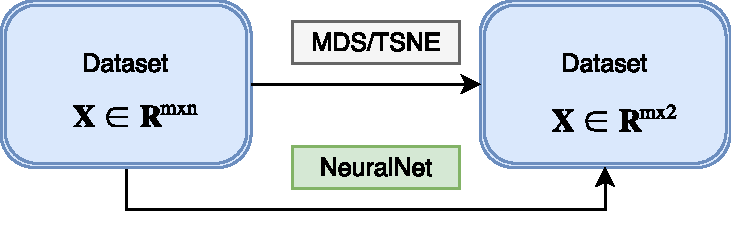
\includegraphics[width=12cm]{figures/neuralnet.pdf}
\caption{\label{figurenet}Dimensionality reduction algorithm learned by a Neural Network}
\end{figure}

\section{Supervised algorithm}
\label{sec:sup}

We have developed a supervised algorithm, based in neural nets, which reproduces the ideas showed in the framework's introduction.
The inputs expected to run this algorithm are the next ones:

\begin{itemize}
\item Number of components for the low-dimensional space
\item Dimensionality reduction object, such as PCA, MDS or TSNE in our examples.
\item Layers: the number of layers and neurons per layer, taking into account that the last layer has the same neurons as the number of components in the low dimensional space; e.g: layers = 2; neurons = 100, 10; it has three layers, with 100, 10 and the number of components neurons each.
\item Dropouts: percentage of neurons from each layer used for training.
\item Learning rate for the neural network training.
\item Activation function for the neural net.
\item Losses function used to minimize the cost.
\item Number of epochs for each training, being epochs the number of times the whole training set has been passed through the neural net.
\item Batch size: number of examples used to compute the gradient of the cost function.
\end{itemize}

The future sections \ref{ssec:nnc}, \ref{ssec:fit} and \ref{ssec:trans} resume some more ideas about the supervised algorithm, describing the construction of the neural net, the fitting process and the dimensionality reduced data obtaining.

\subsection{Neuralnet construction.}
\label{ssec:nnc}

This function is in charge of constructing the neural network taking into account the inputs provided. A neuralnet is defined by the number of layers, number of neurons per layer, activation function, dropouts and loss function. To train the neural net we need to specify the number of epochs and batch size.

\subsection{Fitting process.}
\label{ssec:fit}

The fitting process seeks the parameters or values obtained from a training process given a specific dataset. Depending on whether it is a supervised or non-supervised algorithm, the output of this operations will be either some parameters or directly the remodeled values. For example, as PCA is a parametric transformation, fitting will determine the dimensionality reduction matrix which could afterwards be used to determine the modified data. On the other hand, MDS and TSNE are non-parametric dimensionality reduction algorithms, so the fitting process directly obtains the values from the lower dimension. This parameters and values in the fitting process are stored as an object's own variable until necessary.

We look forward to construct a supervised learning algorithm, based on neural nets, and we want to obtain the parameters learning from the unsupervised embedding algorithm. The steps to take would be as follows: firstly comes the construction of the neural net, taking into account what was said in the previous section plus the input matrix's input. Second of all, we have to store the reduced data from the embedder algorithm. At last, we have the original data and the reduced computed data, so we decided to fit the neural net with both datasets and store the output parameters of the neuralnet.
\vspace{10pt}

\begin{algorithm}
\caption{Fitting process}
\begin{algorithmic}[1]
\Procedure{Fitting Procedure}{}
\State $\textit{\textbf{X}} \gets \text{input matrix}$
\State $ \textit{n\_comp} \gets \text{components in low dimension} $
\BState $\textit{neuralnet} \gets \text{contructed with } \textit{inputs } \text{+ } \textit{\textbf{X}}$
\BState \emph{embedding}
\State $ \textit{\textbf{X\_}} = \text{embedding of } \textbf{\textit{X}}\in R^{mxn} \to R^{mxn\_comp}$
\BState \emph{fit neuralnet}
\State $ out = \text{supervised algorithm, } \textbf{\textit{X}} \to \textbf{\textit{X\_}} $
\EndProcedure
\end{algorithmic}
\end{algorithm}

We have been able to turn a unsupervised learning algorithm into a supervised learning algorithm, by replicating the unsupervised algorithm's behaviour.

\subsection{Dimensionality reduced data obtaining.}
\label{ssec:trans}

We have achieved the task of replicating an unsupervised algorithm's behaviour by a supervised algorithm, characterized for being capable of predicting the output by computing operations between the input and some learned parameters.
Even though the unsupervised algorithms have no parameters, a neural net does. We have obtained, using those parameters, prediction outputs from the new datapoints, which copy the dimensionality reduction without the need to compute the whole algorithm.

\section{Cross Validation}
\label{sec:cv}

Cross validation is a technique to evaluate the predictive models to get to know if the model is capturing the general behaviour of the data to suit the new examples, and moreover estimate how accurate is the model performing.\\
It consists on dividing the data into folds usually depending on the dataset. Choosing between three to five folds would be the best decision. The algorithm is then trained the number folds, using a fraction of disjoint datapoints to train and the rest of them to test. This means in the end we have to test out of sample with all the datapoints. Lastly, a losses metric is used to see how accurate our predictions are. A schema is shown below to represent what cross validation is doing.
\begin{figure}[h]
\centering
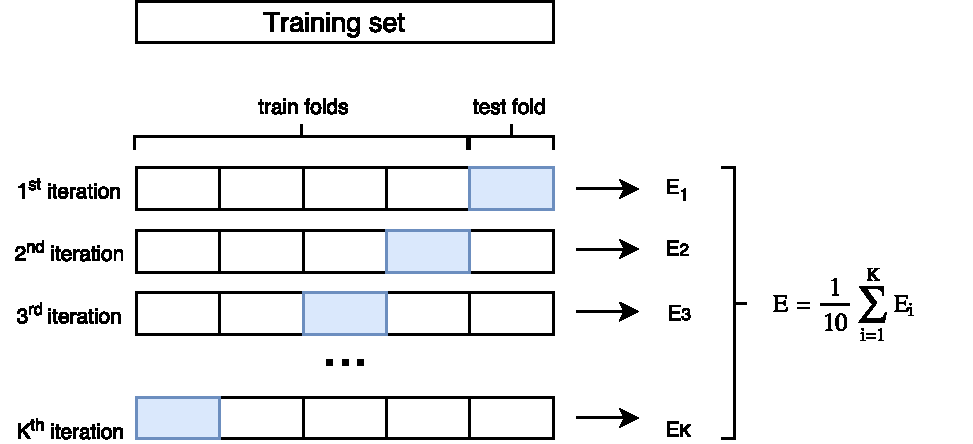
\includegraphics[width=12cm]{figures/cv.pdf}
\caption{\label{figurefit}Cross validation using K-Folds.}
\end{figure}


\section{Metrics}
\label{sec:met}



%-----------------------------------------------------
% Chapter: Applications
%-----------------------------------------------------

\chapter{Applications}
\label{chap:app}

%-----------------------------------------------------
% Chapter: Metrics
%-----------------------------------------------------

\chapter{Metrics}
\label{chap:met}


%-----------------------------------------------------
% Chapter: Conclusion
%-----------------------------------------------------

\chapter{Conclusion}
\label{chap:conc}


%-----------------------------------------------------
% Chapter: Extra
%-----------------------------------------------------

\chapter{EXTRA APPENDIX}
\label{chap:append}

We have developed a class named NNReplicator which replicates the behaviour of a neural net wrapping an embedder object, as it is represented in figure \ref{figurenet}. It is written as if it was a Scikit Learn class so that the objects created could fix into a Scikit Learn pipeline, being one of the main future applications.

Once the inputs are understood, the next point is to get to know what is being computed and what methods are included in the class. As we want to include it as a Scikit Learn class, some methods are required; those are the methods fit and transform, which make the class capable of instantiate tranformers, objects that vary the data input into some output.

It is based on the Keras library, which makes easier the task of programming a neural net. A sequential model is used to stack one layer after the other. We use: add Dense to include a layer, add Activation to specify which activation function to use and add Dropout to include the porcentage of dropout indicated by the corresponding input.\\
The best way of implementing the neural net is by designing a for-loop which extracts the inputs from the arrays and automatically computes denses and dropouts.\\
The default optimizer is Adagrad, and takes as input the learning rate from the object's inicialization. The next step should be the compilation of the whole neural net, using the loss function inputed as the cost to minimize and the model should be completely done.\\
Despite of having built the neural net correctly, we also need to make it compatible with Scikit Learn. That's why the last step consists on a Keras Wrapper, named Keras Regressor, remodeling the model into a sklearn neuralnet model.

%-----------------------------------------------------
% Chapter: Bibliography
%-----------------------------------------------------

\chapter*{Bibliography}
\label{chap:bib}
\addcontentsline{toc}{chapter}{Bibliography}
\bibliography{mybib}
\nocite{*}

% %%%%%%%%%%%%%%%%%%%%%%%%%%%%
% % BIBLIOGRAPHY
% \clearpage
% \phantomsection
% \addcontentsline{toc}{chapter}{Bibliography}
% \bibliography{bib}
% %%%%%%%%%%%%%%%%%%%%%%%%%%%%

%-----------------------------------------------------
% Appendix: Code
%-----------------------------------------------------

\chapter*{Code}
\label{chap:code}
\addcontentsline{toc}{chapter}{Code}

%\begin{tiny}
%\inputminted[baselinestretch=0.5, breaklines]{python}{code.py}
%\end{tiny}

%%%%%%%%%%%%%%%%%%%%%%%%%%%%
% END DOCUMENT
\end{document}
%%%%%%%%%%%%%%%%%%%%%%%%%%%%
